% Editable, one-page US Letter flyer. Compile from this directory:
%   mkdir -p output/pdf
%   xelatex -output-directory=output/pdf Culvert_Workshop_Flyer_Redesigned.tex
% Run xelatex twice on the first build to resolve page anchors.
% Requires TeX Live: fontspec, Inter fonts, graphicx, tikz, hyperref.
% Keep culvert-photo.png, culvert-manual.png, and flyer-assets/ beside this file.
% Content flows within each panel; coordinates below are in PDF points (bp).
\documentclass[letterpaper]{article}
\usepackage[margin=0pt]{geometry}
\usepackage{fontspec,graphicx,tikz}
\usepackage[hidelinks]{hyperref}
\setmainfont{Inter}[Extension=.otf,UprightFont=*-Regular,BoldFont=*-Bold,ItalicFont=*-Italic]
\newfontfamily\semibold{Inter-SemiBold.otf}
\hypersetup{pdftitle={Culvert Vulnerability Assessment Research | Virtual Workshop}}
\definecolor{navy}{HTML}{143442}
\definecolor{ink}{HTML}{263F4C}
\definecolor{teal}{HTML}{227B77}
\definecolor{accent}{HTML}{389B91}
\definecolor{mint}{HTML}{ADD7D1}
\definecolor{pale}{HTML}{EDF4F3}
\definecolor{sidebar}{HTML}{F4F7F8}
\definecolor{muted}{HTML}{58717D}
\definecolor{participate}{HTML}{205C5D}
\pagestyle{empty}
\setlength{\parindent}{0pt}
\setlength{\parskip}{7pt}
\newcommand{\type}[2]{\fontsize{#1}{#2}\selectfont}
\newcommand{\labeltext}[1]{{\type{8}{11}\bfseries\addfontfeatures{LetterSpace=13}#1}}
% Text block: x, y (measured from top left), width, content.
\newcommand{\block}[4]{\node[anchor=north west,inner sep=0pt,outer sep=0pt,text width=#3bp] at (#1,-#2) {\begin{minipage}[t]{#3bp}\setlength{\parskip}{5pt}\raggedright #4\end{minipage}};}
\begin{document}
\noindent\begin{tikzpicture}[remember picture,overlay,x=1bp,y=1bp]
\begin{scope}[shift={(current page.north west)}]
% Hero panel. The photo is cropped to fill the right-hand frame.
\fill[navy] (34,-32) rectangle (578,-195);
\begin{scope}
\clip (371,-35) rectangle (578,-195);
\node[anchor=center,inner sep=0] at (474.5,-115) {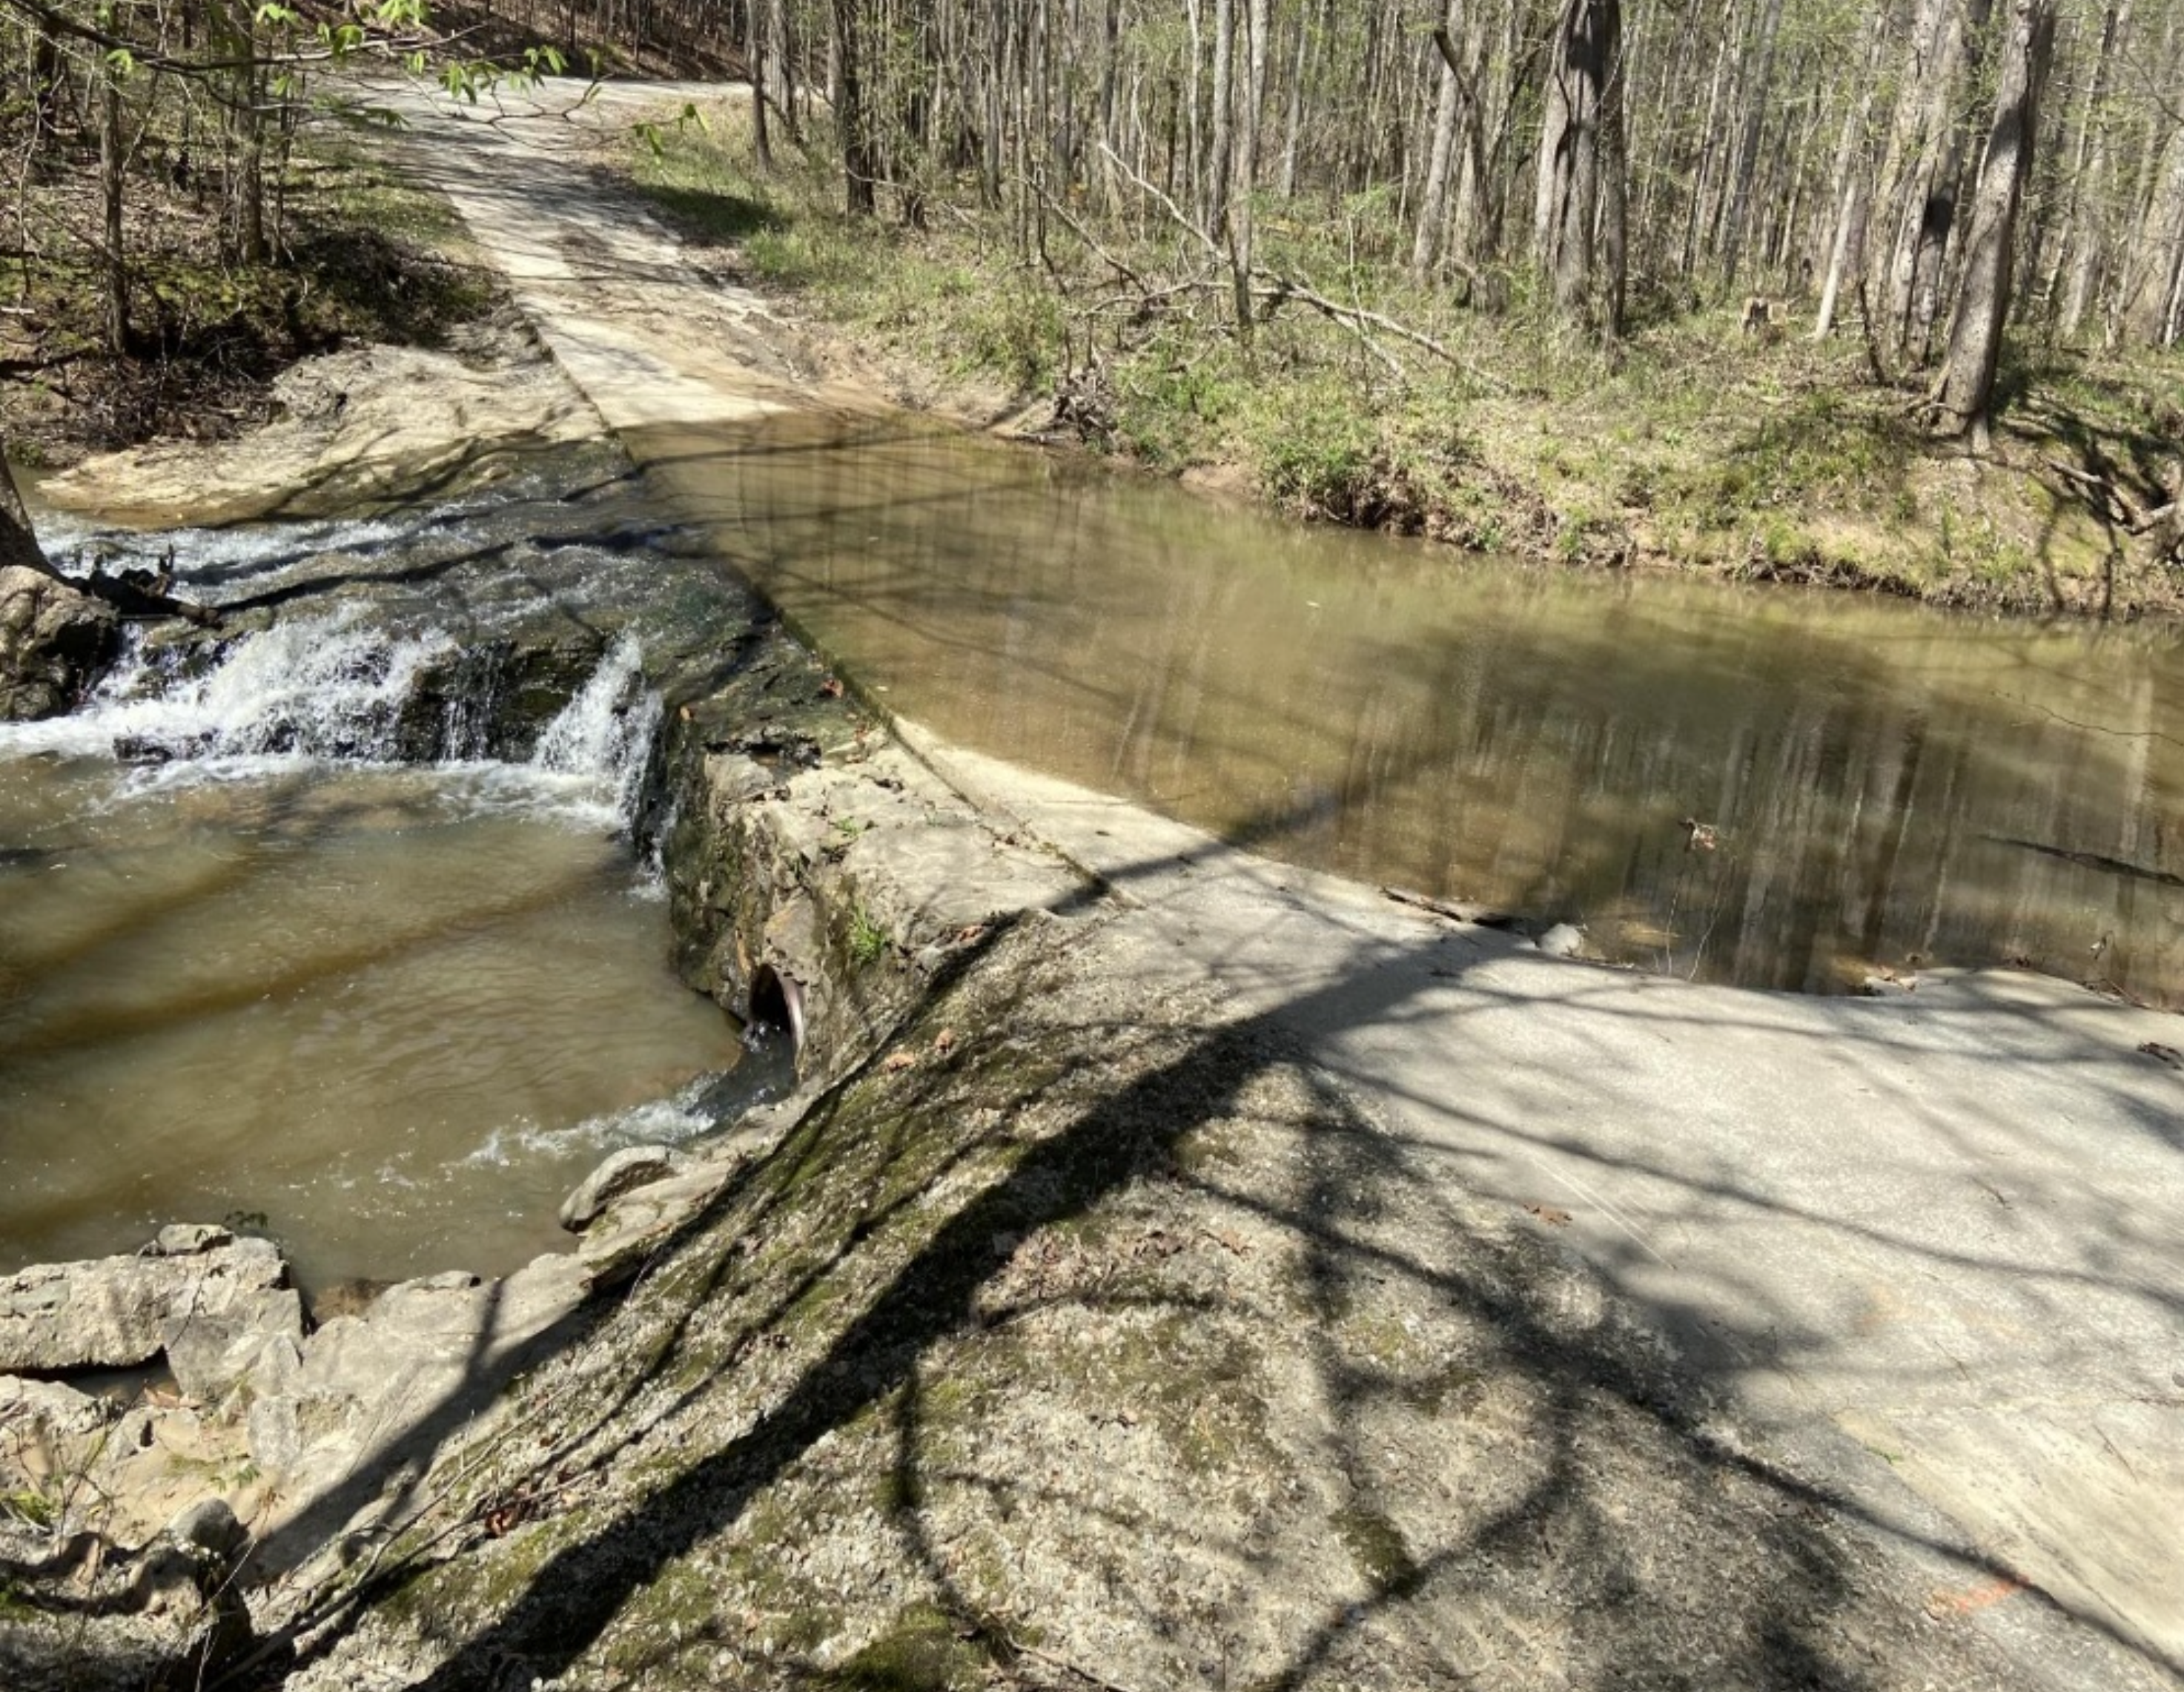
\includegraphics[width=207bp]{culvert-photo.png}};
\end{scope}
\fill[accent] (34,-32) rectangle (578,-35);
\block{54}{52}{310}{\color{mint}\labeltext{VIRTUAL WORKSHOP}}
\block{54}{73}{315}{\color{white}\semibold\type{25}{29}Culvert Vulnerability\\Assessment Research}
\block{54}{143}{310}{\color{white!88!navy}\type{11}{16}Screen forest-road networks.\\Prioritize higher-risk culverts.}
% Date and time panel. Edit the event details here.
\fill[pale] (34,-207) rectangle (578,-292);
\fill[accent] (34,-207) rectangle (37,-292);
\block{51}{219}{400}{\color{navy}\semibold\type{21}{25}December 3, 2026}
\block{477}{227}{91}{\color{muted}\labeltext{3-HOUR SESSION}}
\block{51}{249}{510}{\color{navy}\semibold\type{11.6}{16}1--4 p.m. EST\quad\textcolor{accent}{|}\quad Virtual via Microsoft Teams}
\block{51}{270}{510}{\color{muted}\type{9.1}{12}10 a.m.--1 p.m. PST\quad\textcolor{accent}{\textperiodcentered}\quad11 a.m.--2 p.m. MT\quad\textcolor{accent}{\textperiodcentered}\quad Noon--3 p.m. CT}
% Main column: ordinary editable paragraphs, with automatic line wrapping.
\block{34}{310}{381}{\color{ink}\type{10.3}{15.4}
{\color{teal}\labeltext{ABOUT THE WORKSHOP}}\par
Explore CULVERT, an automated, web-based decision-support tool under continuous expansion, from a multi-phase research collaboration led by the U.S. Forest Service. Its ensemble modeling approach currently helps identify forest-road culverts vulnerable to \textbf{flooding, erosion, and debris flows} before field visits. Coverage of post-wildfire impacts is planned for the near future.\par
Screen large roadway networks and prioritize field inspections, mitigation, design, restoration, and replacement.\par
\vspace{3pt}
{\color{teal}\labeltext{WHO SHOULD ATTEND}}\par
Federal land agency managers, engineers, hydrologists, and researchers.
}
% Participation callout.
\fill[participate,rounded corners=3bp] (34,-495) rectangle (415,-604);
\block{48}{507}{353}{\color{white}\type{10.3}{15}
{\color{mint}\labeltext{PARTICIPATE}}\par
Seeking 2--3 staff from each federal land management agency, plus FHWA staff.\par
{\color{white!85!participate}\type{9.5}{13}Send participant names to:}\\[2pt]
{\semibold\type{11.8}{15}\href{mailto:Brandon.Strohl@dot.gov}{\underline{Brandon.Strohl@dot.gov}}}
}
% Resource sidebar. Both the cover and website text are clickable.
\fill[sidebar] (435,-310) rectangle (578,-605);
\block{447}{323}{119}{\centering\color{teal}\labeltext{EXPLORE THE TOOL}}
\node[anchor=north west,inner sep=0] at (461,-344) {\href{https://culvert-at-risk.org/}{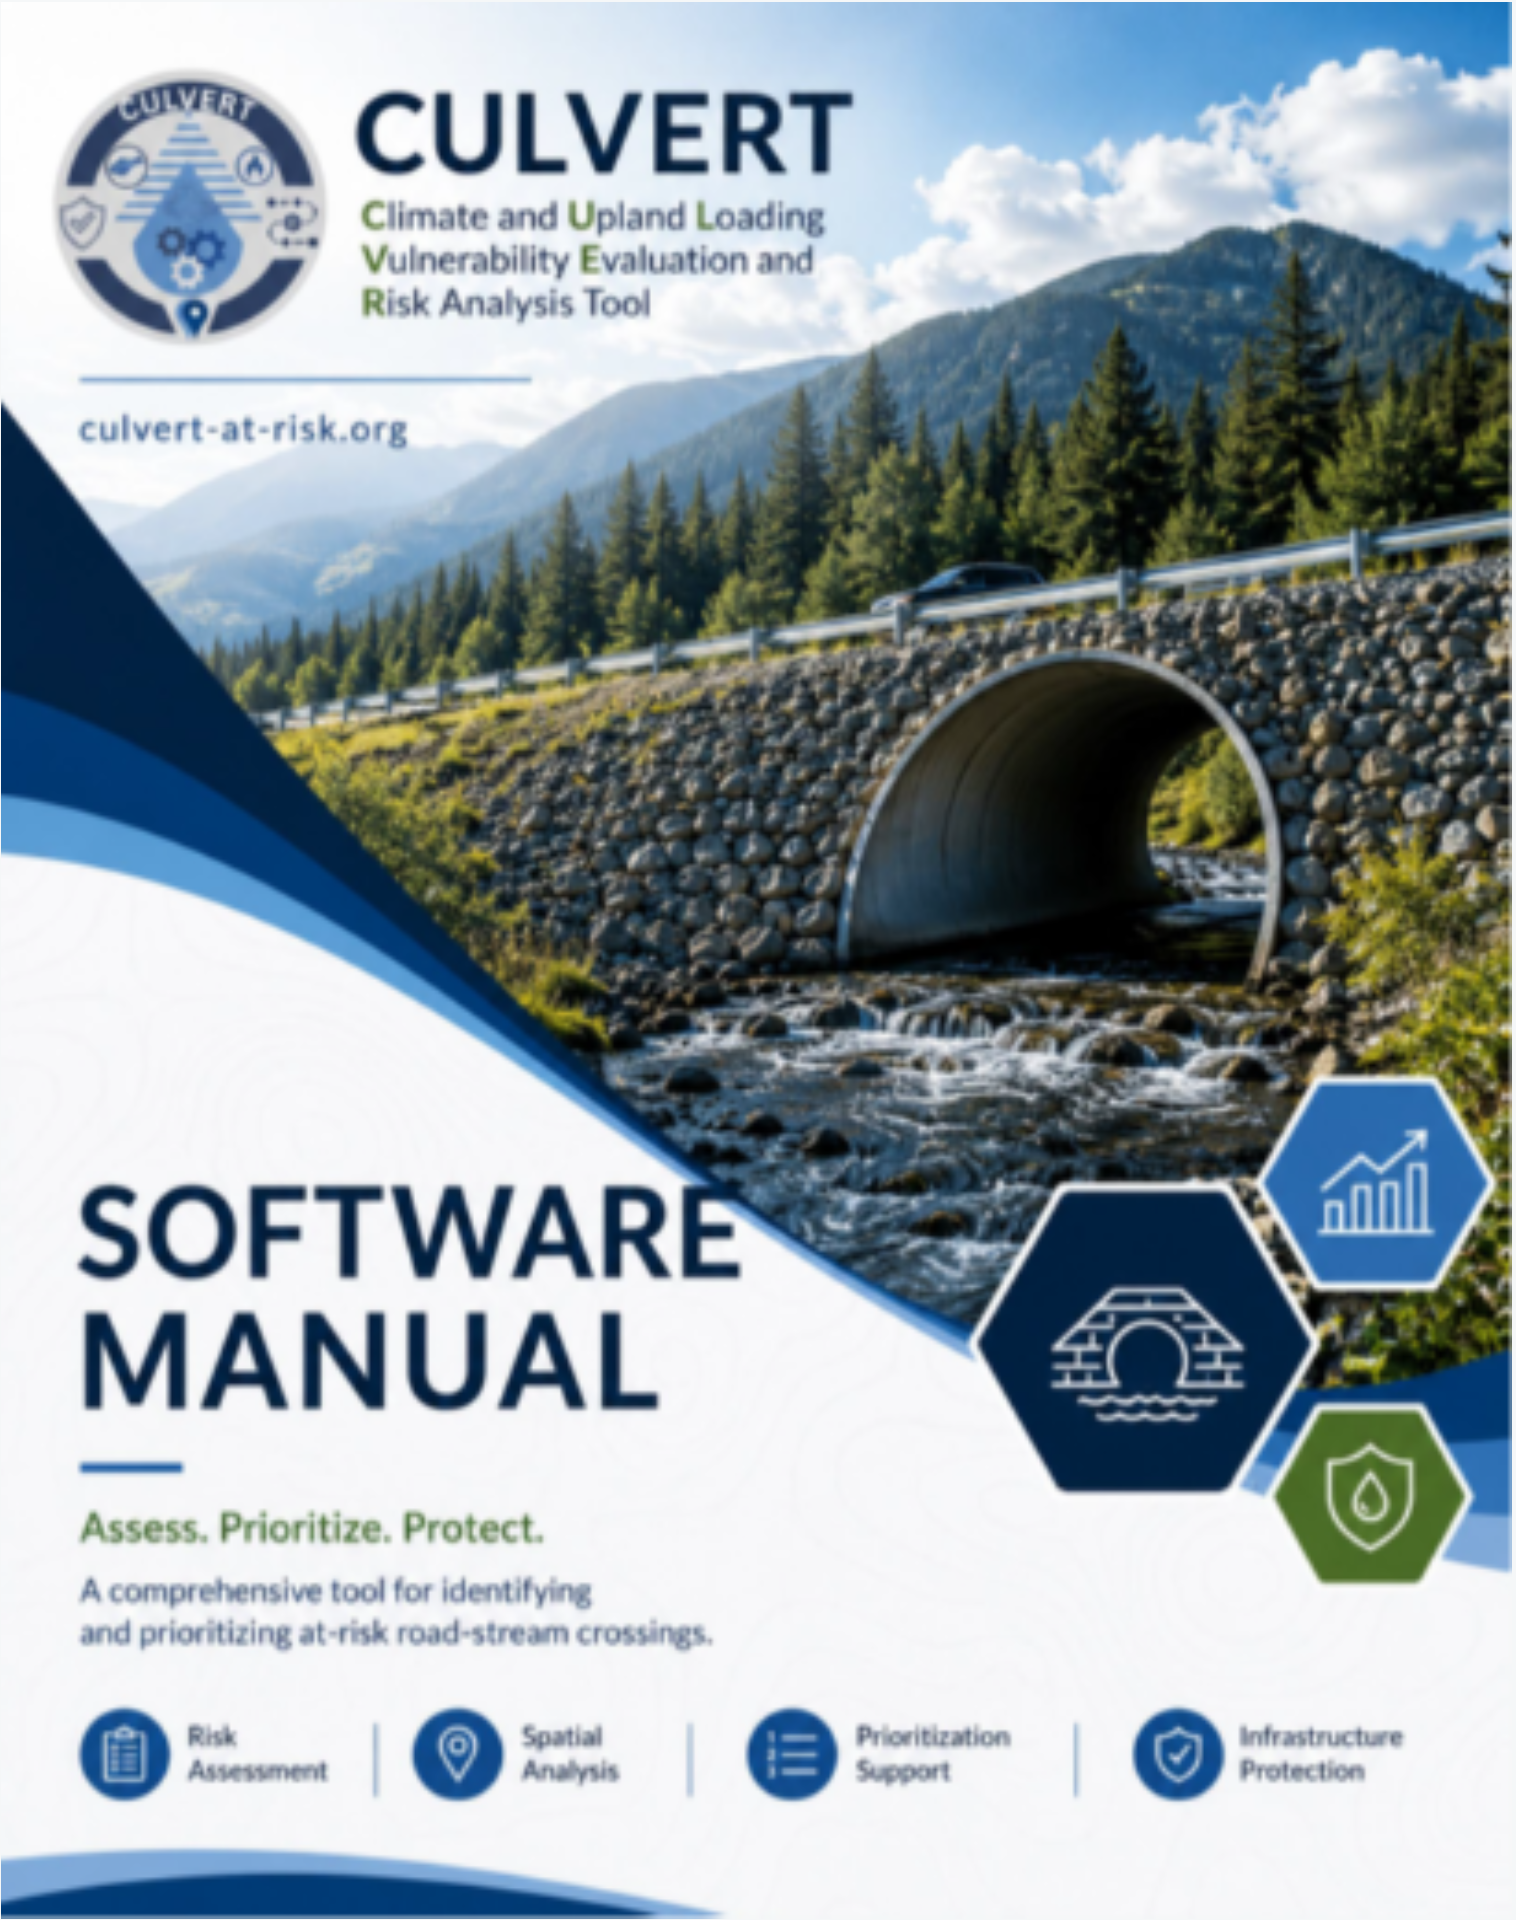
\includegraphics[width=91bp]{culvert-manual.png}}};
\block{447}{472}{119}{\color{teal}\semibold\type{10.3}{14}\href{https://culvert-at-risk.org/}{\underline{culvert-at-risk.org}}\par
\normalfont\color{muted}\type{8.5}{12}CULVERT project website}
\draw[muted!25,line width=.6bp] (447,-512) -- (566,-512);
\block{447}{523}{119}{\color{teal}\type{9.3}{13.7}\href{https://research.fs.usda.gov/srs/projects/culvert-resilience-tool}{\underline{Culverts for climate}\\\underline{resilience: Developing the}\\\underline{CULVERT tool}}\par
\color{muted}\type{8.5}{12}U.S. Forest Service\\Research \& Development}
% In-person event and partner marks.
\draw[muted!35,line width=.8bp] (34,-622) -- (578,-622);
\block{34}{635}{544}{\color{teal}\labeltext{IN-PERSON OPPORTUNITY · TRB ANNUAL MEETING}}
\block{34}{651}{544}{\color{navy}\semibold\type{10.5}{15}Sunday, January 10, 2027\quad\textcolor{accent}{|}\quad1:30--4:30 p.m.\quad\textcolor{accent}{|}\quad Washington, DC}
\block{34}{672}{544}{\color{muted}\type{9}{13}A version of this workshop is on the agenda during the January 10--14, 2027 TRB Annual Meeting at the Walter E. Washington Convention Center and Marriott Marquis.}
\node[anchor=north,inner sep=0] at (174,-711) {
\includegraphics[height=48bp]{flyer-assets/forest-service.png}};
\node[anchor=north,inner sep=0] at (262,-711) {
\includegraphics[height=49bp]{flyer-assets/transportation.png}};
\node[anchor=north,inner sep=0] at (350,-711) {
\includegraphics[height=49bp]{flyer-assets/north-georgia.png}};
\node[anchor=north,inner sep=0] at (438,-711) {
\includegraphics[height=49bp]{flyer-assets/idaho.png}};
\end{scope}
\end{tikzpicture}
\null
\end{document}
